\chapter{Provoz}
\label{ch:provoz}

Následující kapitola shrne možnosti realizovaného rozšíření pro koordinaci IoT, popíše, jaké je použití pro provoz
sítě Internetu věcí a poté ověří realizované prostředky pro koordinaci IoT na produkčním příkladu.

\section{Nasazení a provoz systému}\label{sec:nasazení-a-provoz-systému}
Pro běh systému s~realizovaným rozšířením bylo nutné zajistit následující prostředky:
\begin{itemize}
    \item \textbf{Server} \\
    Pro běh požadovaných komponent celého systému je požadován server, ke kterému se budou schopny uzly pomocí
    bezdrátové sítě připojit a bude schopen provozovat běhové prostředí Node.js -- v~použitém příkladu se bude jednat
    o~VPS s~operačním systémem Debian.

    \item \textbf{Běhové prostředí pro nástroj Node-RED} \\
    Vzhledem k~ekosystému nástroje Node-RED byl zvolen nástroj PM2\footnote{\url{http://pm2.keymetrics.io/}}, který pro
    aplikace v~programovacím jazyce Javascript zajišťuje správu jejich běhu, tj. monitorování použitých systémových
    prostředků, jejich programové smyčky událostí či paralelní běh -- pro správce systému poskytuje možnost Node-RED
    spustit.

    \item \textbf{Broker MQTT} \\
    Jako broker byla zvolena implementace s~názvem \emph{Eclipse Mosquitto}\footnote{\url{https://mosquitto.org/}} --
    jedná se o~nástroj s~otevřeným zdrojovým kódem od společnosti Eclipse.
    Broker dle dokumentace podporuje všechny z~požadovaných vlastností (parametr zprávy \uv{retain}, tři úrovně QoS,
    zprávu poslední vůle atd.) a je dostupný jako aplikační balíček pro použitý operační systém.

    \item \textbf{Moduly ESP32} \\
    Pro produkční použití byly použity moduly ESP32 s~deskou plošných spojů obsahující stabilizátor napětí, převodník
    UART-USB a lištu pinů umožňující zapojení do nepájivého pole -- jedná se o~moduly s~produktovým názvem
    \uv{ESP32-DevKitC}\footnote{\url{https://www.espressif.com/en/products/hardware/esp32-devkitc/overview}}
    přímo od firmy Espressif Systems.
\end{itemize}

Všechny výše uvedené prostředky jsem použil pro sestavení vlastního lokálního Internetu věcí, nad kterým jsem následně
prováděl experimenty a ověřoval funkci realizovaných prostředků.
Postup spuštění toto systému byl následující:
\begin{enumerate}
    \item \textbf{Instalace firmwaru na uzel} \\
    Pro realizované programové vybavení pro uzly ESP32 existuje také instalátor v~podobě předpisu pro standardní
    utilitu \texttt{make} -- instalace je složena ze tří hlavních kroků (více k~tomuto postupu je uvedeno
    v~příloze~\ref{ch:instalator}).
    Prvním krokem je zavedení samotného interpretu jazyka MicroPython, následuje instalace externích knihoven jakožto
    závislostí realizovaného firmwaru a následně samotný kód firmwaru.
    Po ověření funkce firmwaru je posledním krokem zapnutí automatického zavedení firmwaru při startu -- uzel je v~tu
    chvíli připraven pro provoz čistě přes internetové připojení.
    Výstupem instalace je, kromě pro provoz připraveného uzlu, unikátní identifikátor uzlu, který bude následně použit
    pro zacílení ze strany nástroje Node-RED.

    \item \textbf{Instalace Node-RED rozšíření} \\
    Pro instalaci vlastního rozšíření do tohoto nástroje je nutné dodržet požadavky popsané
    v~\ref{sec:node-red-rozsireni} -- realizované rozšíření všechny tyto formální požadavky splňuje, je tedy možné jej
    nainstalovat do jmenného prostoru knihoven nástroje Node-RED, například pomocí nástroje \texttt{npm}.
    Ve chvíli startu si tento nástroj knihovny poskytující bloky zaregistruje do galerie bloků, které následně nabízí
    uživateli.

    \item \textbf{Příprava sítě} \\
    Dalším krokem je příprava samotné sítě v~nástroji Node-RED, jedná se o~postupně o~výběr bloků pro síť (senzory,
    rozhodovací prvky, výstupní prvky), jejich nastavení (použité piny na uzlu, podmínky, rozmístění prvků v~GUI)
    včetně konfiguračních bloků (broker MQTT, identifikace uzlů získané při instalaci) a na závěr jejich propojení do
    sítě pomocí datových spojů.
    Příklad sítě, která s~pomocí senzoru DHT měří teplotu a vlhkost místnosti, kterou
    exportuje do uživatelského rozhraní, je vyobrazen na obrázku~\ref{fig:node-red-production-1}
    Proces přípravy sítě je zakončen jejím nasazením -- editor zašle konfiguraci do běhové části nástroje, jenž provede
    reinicializaci sítě a jejích bloků.
\end{enumerate}

\section{Scénáře užití}\label{sec:scenare-uziti}

Pro ověření funkce systému byly použity dva případy užití, které budou představeny v~následujících kapitolách -- vždy
textový popis případu užití, zobrazení implementace sítě v~nástroji Node-RED a ukázka ze sestaveného uživatelského
rozhraní.

\subsection{Měření prostředí v~místnosti s~výstupem do uživatelského rozhraní}\label{subsec:scenar-1}

Síť prvního scénáře obsahuje vstupní blok reprezentující senzor typu DHT22 měřící teplotu a vlhkost okolního prostředí.
Zprávy z~tohoto senzoru odečítá nasazená aplikace na uzlu s~intervalem 30 sekund a skrz firmware a broker MQTT je
distribuuje do sítě nástroje Node-RED, kde jsou dále zpracovávány -- dojde
k~vyextrahování hodnoty teploty a vlhkosti ze zprávy, zobrazení aktuální hodnoty v~textovém výstupu uživatelského
rozhraní a promítnutí časového aritmetického průměru hodnoty za 15 minut do grafu.

Implementace sítě pro tento scénář je zobrazena v~obrázku~\ref{fig:node-red-production-1}, odpovídající část
uživatelského rozhraní je poté vyobrazena na obrázku~\ref{fig:node-red-production-1-ui}.

\begin{figure}
    \centering
    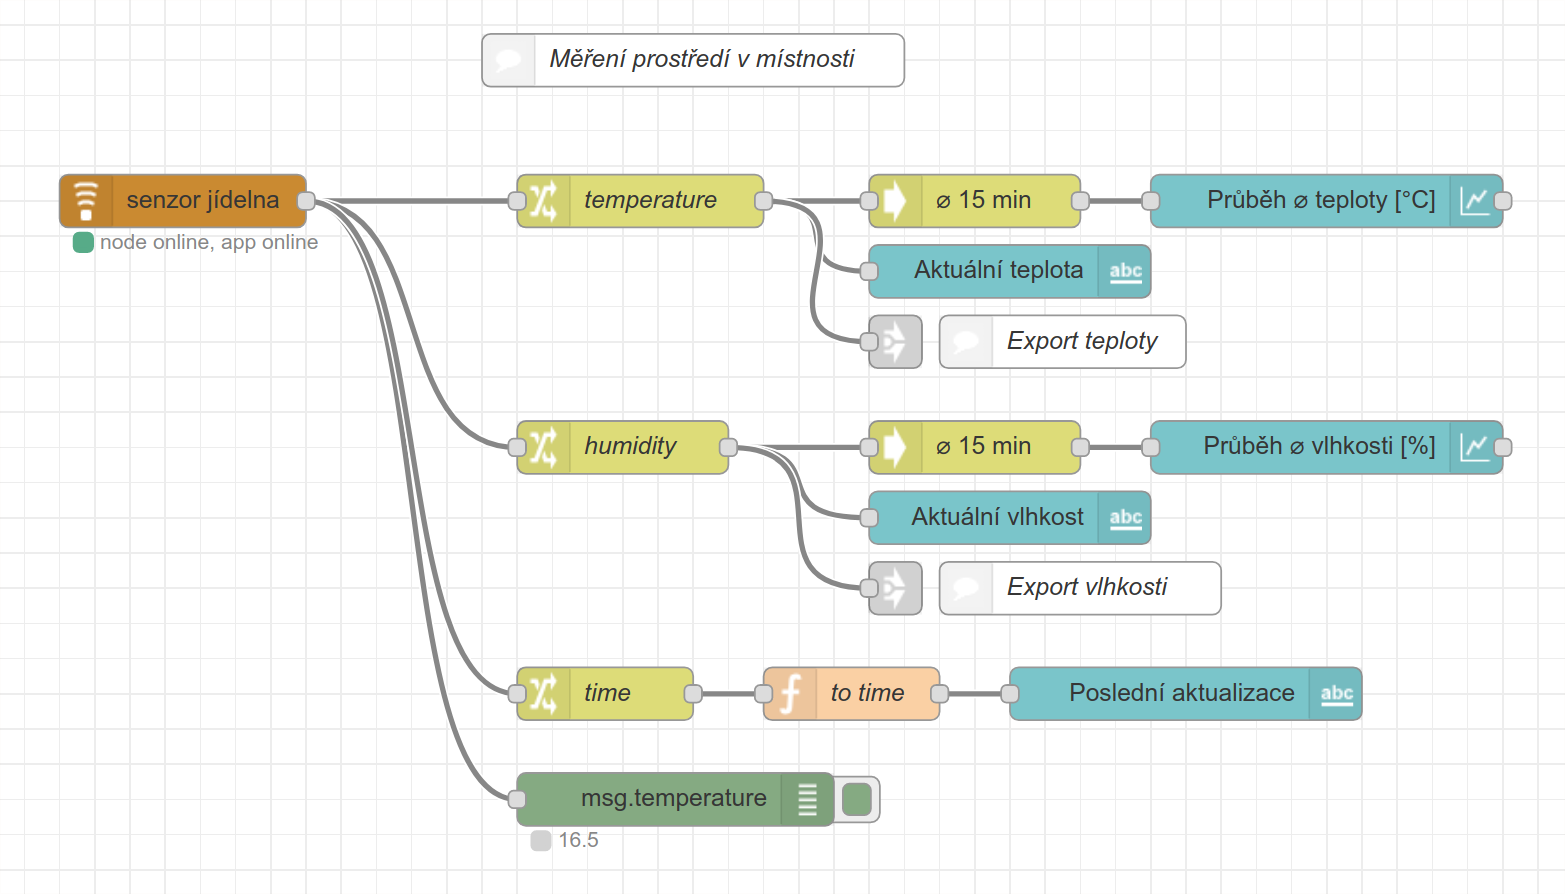
\includegraphics[width=\textwidth]{figures/fis-flow-1.png}
    \caption{Implementace sítě pro scénář  \textit{Měření prostředí v~místnosti s~výstupem do uživatelského
    rozhraní} -- vlevo se nachází vstupní blok reprezentující uzel s~připojeným senzorem typu DHT22.
    Výstup tohoto bloku dále směřuje do bloků exportující konkrétní hodnoty ze zprávy (vstupem je datový typ
    \ic{Object}, výstupem \ic{float}), ze kterých již dochází k~zobrazení a vyhodnocení časového aritmetického
    průměru pro graf -- pro snažší ladění je zde přidán blok typu \texttt{debug}, který exportuje aktuální teplotu
    do ladícího panelu nástroje.
    Pro signalizaci času poslední aktualizace slouží soustava bloků pro nastavení aktuálního času při přijetí zprávy
    a jeho konverze na podobu do uživatelského rozhraní.}
    \label{fig:node-red-production-1}
\end{figure}
\begin{figure}
    \centering
    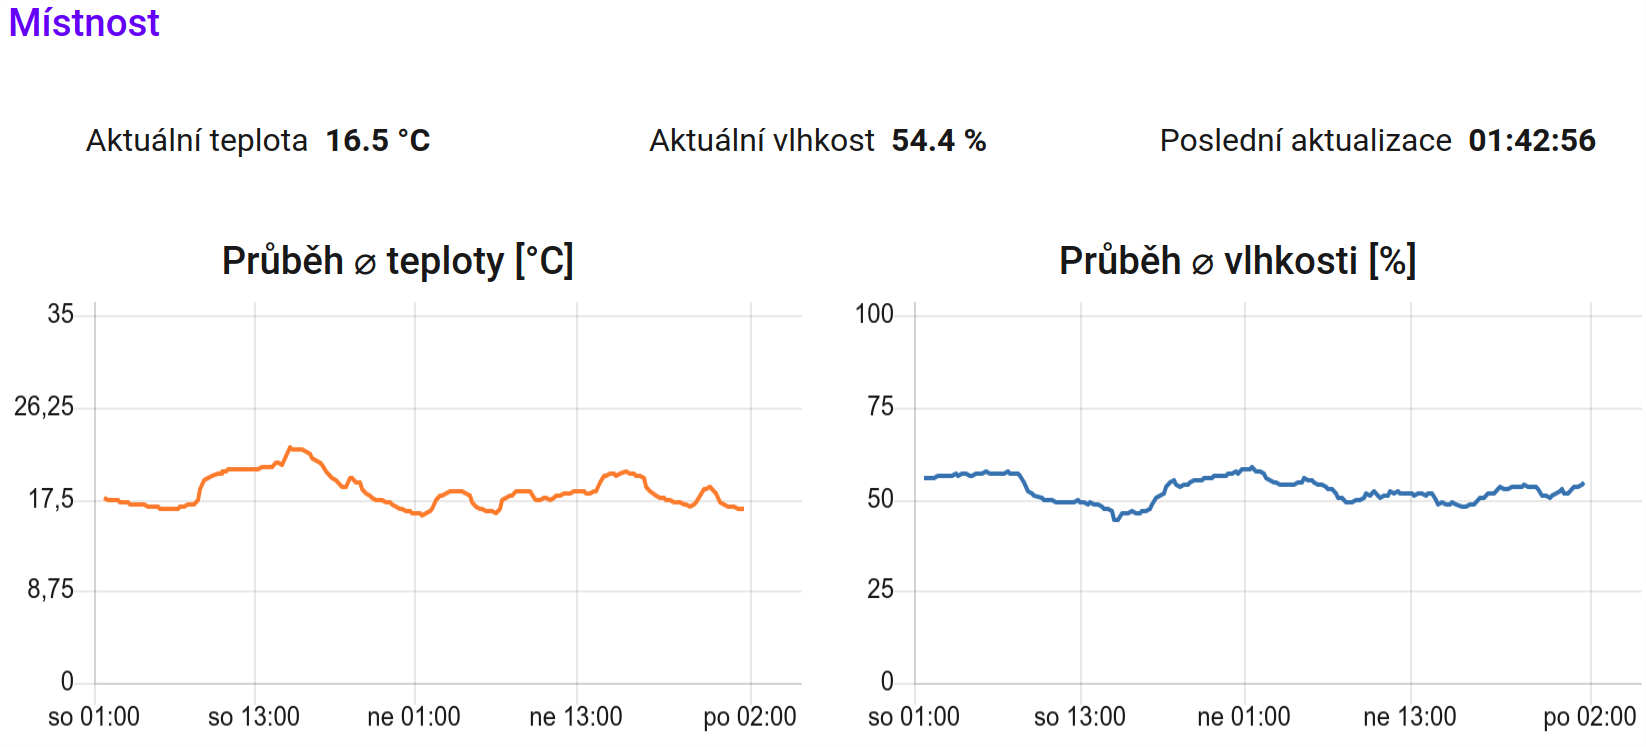
\includegraphics[width=\textwidth]{figures/fis-flow-1-ui.png}
    \caption{Ukázka z~uživatelského rozhraní pro scénář \textit{Měření prostředí v~místnosti s~výstupem do
    uživatelského rozhraní} -- kromě naposled změřených hodnot se zde nachází grafy průběhů měřených hodnot a čas
    poslední aktualizace.}
    \label{fig:node-red-production-1-ui}
\end{figure}

\subsection{Zobrazení aktuálního času a teploty na displeji}\label{subsec:scenar-2}

Druhý testovací scénář obsahuje displej sestavený z~LED diod technologie Neopixel, na který se zobrazuje aktuální čas
a aktuální teplota v~měřené místnosti z~prvního scénáře -- čas je vždy zobrazen po dobu $X$ a následně je po dobu $Y$
zobrazena teplota.
Tyto hodnoty jsou uživatelem stanoveny z~uživatelského rozhraní -- v~implementaci sítě tedy běží čítač, který na
základě předaných vstupů definuje výstup do displeje.
Speciálním případem je zadání statického textu do rozhraní, tento text je poté zobrazen bez vlivů čítače -- ve všech
případech lze použít vstup pro výběr požadované barvy displeje.

Ukázka z~implementace této sítě se nechází na obrázku~\ref{fig:node-red-production-2}, sestavené uživatelské rozhraní
poté na obrázku~\ref{fig:node-red-production-2-ui}.

\begin{figure}
    \centering
    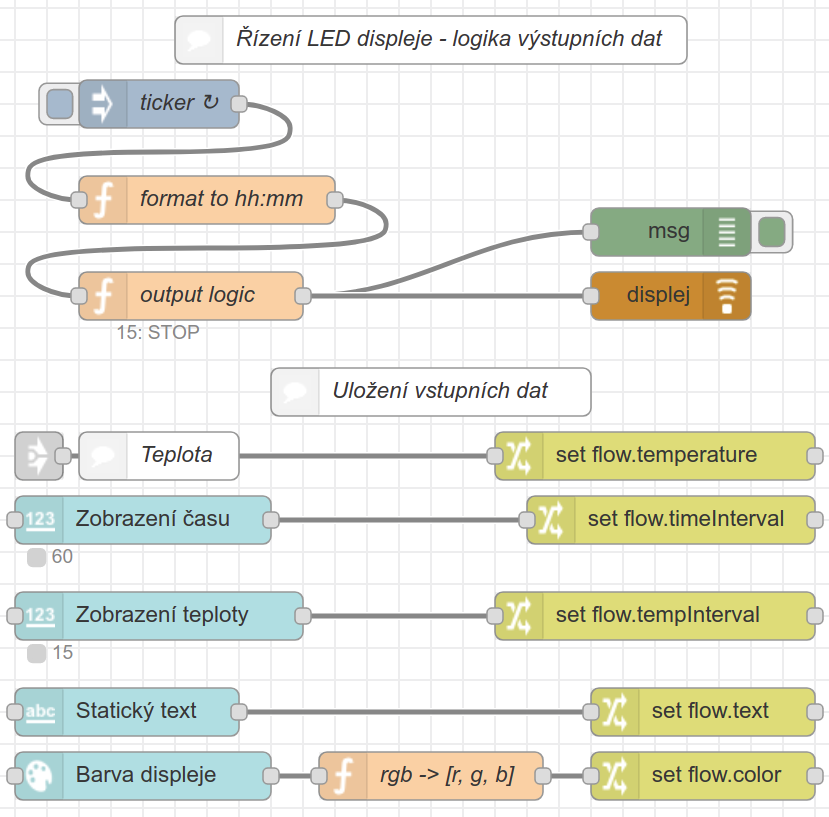
\includegraphics[width=.7\textwidth]{figures/fis-flow-2.png}
    \caption{Implementace sítě pro scénář \textit{Zobrazení aktuálního času a teploty na displeji} -- funkce je
    založena na dvou částech.
    Spodní část je určena k~ukládání aktuální stavu nastavení, tedy testického textu, intervalů zobrazení a pomocí
    tunelového spojení i aktuální teploty -- využito je k~tomu vlastnosti nástroje umožňující uložení informace
v~rámci jedné sítě.
    Horní část poté obsahuje časovač, který invokuje vlastní implementaci rozhodovací logiky, jejíž výstupem je
    zpráva směrovaná do blok displeje (a pro snažší ladění i do postranního panelu).}
    \label{fig:node-red-production-2}
\end{figure}
\begin{figure}
    \centering
    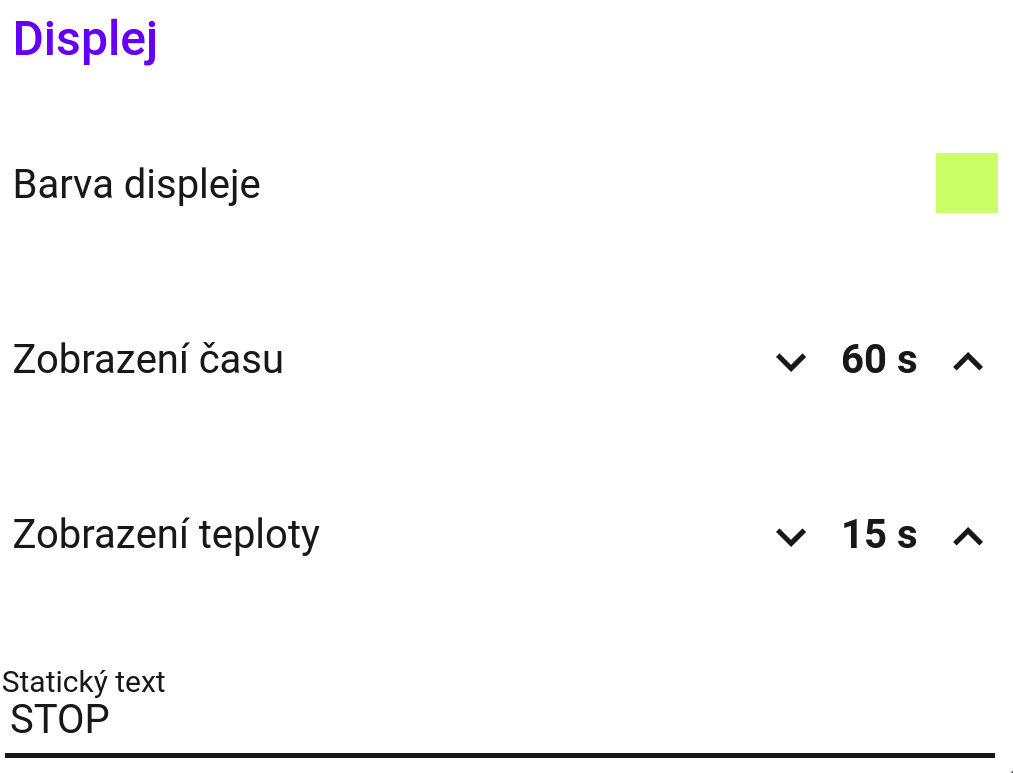
\includegraphics[width=.5\textwidth]{figures/fis-flow-2-ui.png}
    \caption{Ukázka z~uživatelského rozhraní pro scénář \textit{Měření prostředí v~místnosti s~výstupem do
    uživatelského rozhraní} -- kromě naposled změřených hodnot se zde nachází grafy průběhů měřených hodnot a čas
    poslední aktualizace.}
    \label{fig:node-red-production-2-ui}
\end{figure}

\section{Vyhodnocení provozu scénářů}\label{sec:vyhodnocení}

Oba scénáře byly po dobu sedmi dnů provozovány paralelně na dvou samostatných uzlech.
Během této doby se realizovanému \textbf{systému plně dařilo vykonávat zadanou funkci} -- firmware uzlu se vypořádal
s~lokálně slabým a nestabilním signálem bezdrátové sítě pomocí procesu znovupřipojení k~internetu a brokeru.
Výsledkem bylo obnovené spojení, díky kterému obdržel uzel od brokeru poslední konfigurační data a data pro
aplikace.
Z~těchto dat zreprodukoval vnitřní stav a výstupy či vstupy -- zobrazený text v~případě displeje či naplánované měření
v~případě senzoru.
Toto chování bylo autorem zjištěno pomocí manuálního připojení se na konzoli uzlů přímo v~místě.

V~této době bylo také odpozorováno několik automatických restartů uzlů, příčin bylo postupně několik -- nedostatek
paměti při zavedení většího množství aplikací na uzel během testování, zvýšený výkonnový odběr uzlu v~případě
displeje bez externího zdroje a tím i zapříčiněný pád operačního systému pro nedostatek energie v~procesoru nebo
stav, kdy dojde k~uzavření spojení MQTT ze strany brokeru, a tím i automatickému restartu uzlu.

\textit{Oba scénáře používaly každý samostatně svůj vlastní fyzický uzel -- pro navržený systém by ovšem nebyl
problém provozovat oba scénáře na jednom uzlu vedle sebe, jak bylo autorem ověřeno během experimentů.}